\documentclass[11pt]{article}
\usepackage{geometry}                
\geometry{letterpaper}                 
\usepackage[parfill]{parskip}        
\usepackage{graphicx}
\usepackage{amssymb}
\usepackage{amsmath}
\usepackage{epstopdf}
\usepackage{verbatim}
\usepackage{float}
\usepackage{enumerate}
\usepackage{hyperref}
\usepackage[utf8]{inputenc}
\usepackage[T1]{fontenc}
\DeclareGraphicsRule{.tif}{png}{.png}{`convert #1 `dirname #1`/`basename #1 .tif`.png}
\usepackage{color}
\usepackage{textcomp}
\definecolor{listinggray}{gray}{0.9}
\definecolor{lbcolor}{rgb}{1,1,1}

\begin{document}

\section*{Problems for Discussion 2, 09/18/13}
Compiled by Mai Le, some problems from Prof. Fessler
% $x[n]$ can refer to a sequence or a value

\section{Discrete-domain Basis Sequences}
Let $x[n] = \{\underline{1},1,2,3,5\}$. Represent $x[n]$ in each of the following bases. 

Note: You won't be asked to do anything like this on the homework or exams, but hopefully it will help you solidify your understanding of bases from lecture.

\subsection*{Unit Step Sequences}
Recall $u[n] = \begin{cases}1, & n \geq 0\\ 0, & n < 0 \end{cases}$. Let $\mathcal{S}_u = \{u[n-n_0]|n_0 \in \mathbb{Z}\}$ (unit steps shifted by any integer $n_0$) be your basis sequences. Represent $x[n]$ in $\mathcal{S}_u$.

In other words, show you can write $x[n]=\sum\limits_{k=-\infty}^\infty c_k u[n-k]$ by finding the values for $c_k$.

\subsection*{Three-Tap Rectangles}
Let $r[n] = \{\underline{1},1,1\}$ and $\mathcal{S}_r = \{r[n-n_0]|n_0 \in \mathbb{Z}\}$. Represent $x[n]$ in $\mathcal{S}_r$.

\subsection*{Three-Tap Triangle}
Let $t[n] = \{\underline{1},2,1\}$ and $\mathcal{S}_t = \{t[n-n_0]|n_0 \in \mathbb{Z}\}$. Represent $x[n]$ in $\mathcal{S}_t$.

\section{Properties of Even More Systems}
Are the following linear? time-invariant? causal? stable?

\subsection*{(a)}

$y[n] = x^2[n+1]$

\subsection*{(b)}

$y[n]=\begin{cases}x[-n], & n < 0\\ x[n], & n \geq 0 \end{cases} $

\subsection*{(c)}

$y[n] = \sum_{k=-\infty}^{\infty}x[n-k]p[k]$ where $p[n] = \{-10,\ldots,-1,\underline{0},1,\ldots,10\}$.

%\section{Decomposition of Signals into Even and Odd} 

\section{Proof of Parseval's Theorem}
Prove that $\sum_{n=-\infty}^\infty|x[n]|^2 = \frac{1}{2 \pi} \int_{- \pi}^\pi |X(\omega)|^2 d\omega$.

\section{Orthogonality of Complex Exponentials}

\subsection*{(a)}
Prove $\frac{1}{N}\sum\limits_{n=0}^{N-1} e^{j\frac{2 \pi}{N} k n} = \begin{cases}1, & k =0, \pm N, \pm 2N,... \\0, & otherwise \end{cases}$.

\subsection*{(b)} 
Show that harmonically related complex exponential signals $s_k[n]=e^{j\frac{2 \pi}{N} kn}$ are orthogonal over any interval of length $N$. I.e. $\sum\limits_{n=n_0}^{n_0+N-1} s_k[n]s_l^*[n] = 0$ if $k \neq l$.

\section{Symmetry and the DTFT}
\subsection*{(a)}

Let $y[n] = x^*[-n]$. What is $Y(\omega)$ in terms of $X(\omega)$?

\subsection*{(b)}

If $x[n]$ is real, what can we say about the symmetry of $X(\omega)$?

\section{Inverse DTFT}
\subsection*{(a) Inverse DTFT of a Triangle}
Find the signal $x[n]$ that has the following spectrum. Hint: integration by parts!

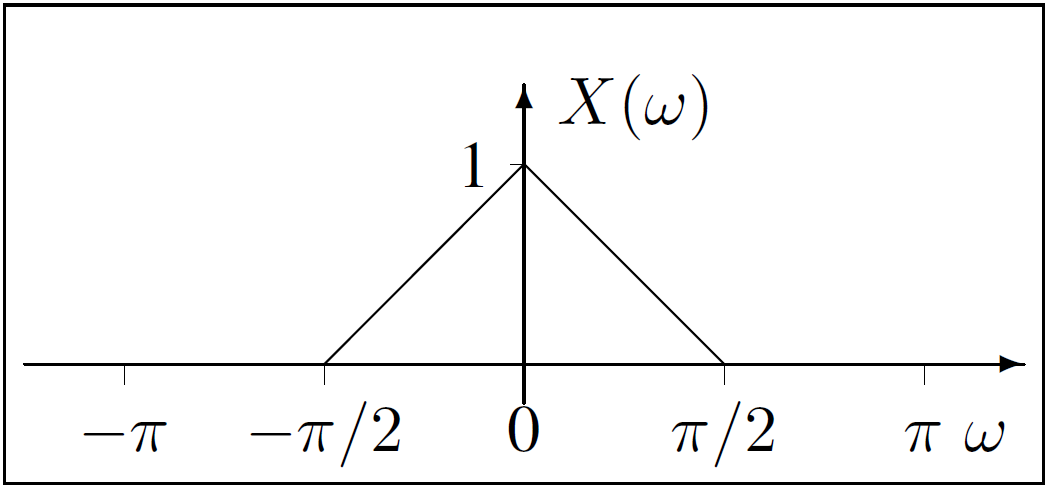
\includegraphics[scale=0.25]{fessler_hmwk6_p1.png}

\subsection*{(b)}
Given: $h[n] = \delta[n-1]+\delta[n+1]$ has spectrum $H(\omega) = 1 e^{-j\omega}+1e^{j\omega}=2cos(\omega)$. (You should be able to verify this.)

Find the signal $y[n]$ that has the spectrum $Y(\omega)=cos^2(\omega)$. (Don't do the integration!)


\section{Inverse DTFT}
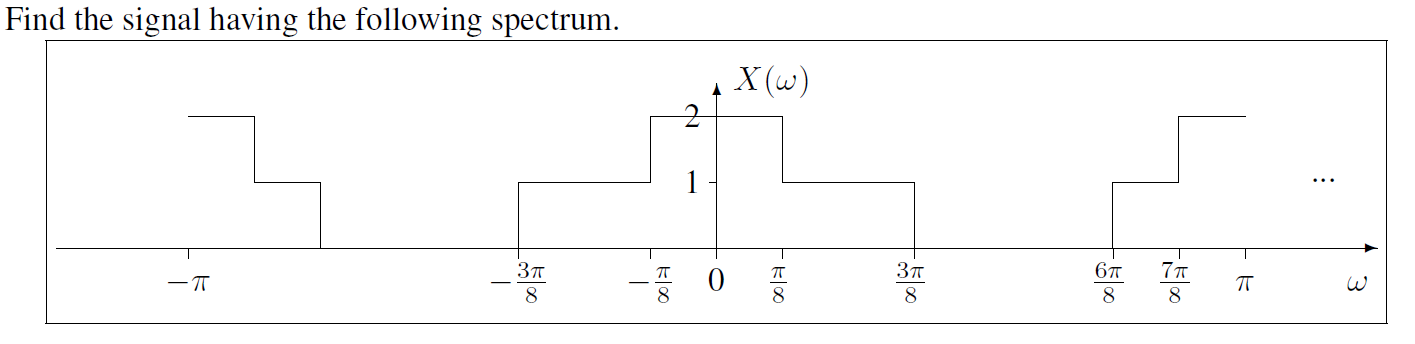
\includegraphics[width = \textwidth]{fessler_hmwk5_p9.png}

\end{document}